\section{Theorie} 
\label{sec:Theorie}

In diesem Kapitel werden die theoretischen Hintergründe dieses Versuches erläutert. Dabei wird insbesondere auf die in der Durchführung verwendeten Schaltungen eingegangen.
\subsection{Das Bändermodell}
\label{sec:baendermodell}
Ein einzelnes Atom besitzt nur diskrete Energiniveaus auf denen sich Elektronen befinden können. In einem 
Festkörper dürfen die Energieniveaus der Atome allerdings nicht vollständig gleich sein und unterscheiden sich 
daher minimal, sin aber dennoch nah genug beieinander das die Elektronen problemlos zwischen den Niveaus 
wechseln können, sie sind quasikontinuirlich. So ergeben sich die sogenannten Bänder. Bänder die vollständig 
mit Elektronen gefüllt sind tragen nicht zur elektrischen Leitfähigkeit bei, sie heißen Valenzbänder. 
Die Bänder sind im Energieraum ausgedehnt und können sich mit anderen Bändern überschneiden, oder durch eine 
Bandlücke voneinander getrennt sein. Bei einer großen Bandlücke und keinen Elektronen im Leitungsband
ist der Stoff ein Isolator. Hier ist die Bandlücke so groß das auch bei hohen Temperaturen keine nennenswerte Zahl
von Elektronen in das Leitungsband aufsteigen kann und so auch bei hohen Temperaturen keine elektrische
Leitfähigkeitentsteht. Bei einer schmalen Bandlücke ist der Stoff ein Halbleiter. Hier können durch thermische 
Anregung genug Elektronen ins Leitungsband aufsteigen um elektrische Leitfähigkeit zu gewährleisten. Am absoluten
Nullpunkt leiten intrinsische Halbleiter keinen Strom.
\begin{figure}
    \centering
    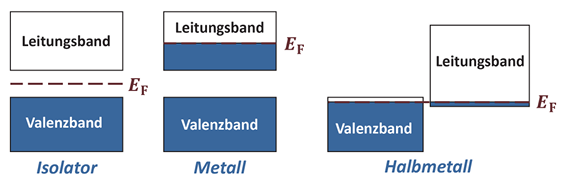
\includegraphics[width=1\textwidth]{content/grafiken/baender.JPG}
    \caption{Vergleich der Bändermodelle von Isolatoren, Leitern und Halbleitern. $E_F$ bezeichnet die Fermienergie [1]}
    \label{fig:baendermodell}
  \end{figure}
\subsection{Die effektive Masse}
\label{sec:effektiveMasse}
Elektronen können sich auch im Festkörper nicht als vollständig frei betrachtet werden. Sie spüren die 
ortsabhängigen Potentiale der Atomrümpfe. Daher wird die effektive Masse $m^{\star}$ eingeführt. 
Dank ihr können die Elektronen in Leitungs- und nicht vollständig besetztden Valenzbändern als freie Elektronen
mit der Dispersionsrelation
\begin{equation}
  \label{eq:dispersionsrelation}
  E(\vec{k})=E_0+\frac{\hbar^2k^2}{2m^{\star}}
\end{equation}
beschrieben werden. Dabei ist $m^{\star}$ durch 
\begin{equation}
  m^{\star}=\hbar(\frac{\mathrm{d}^2E}{\mathrm{d}k_i\mathrm{d}k_j})^{-1}
\end{equation}
gegeben.
\subsection{Dotierung}
\label{sec:dotierung}
Reine Halbleiter, die auch als intrinsisch bezeichnet werden, leiten zwar elektrischen Strom, allerdings nicht
besonders gut. Daher werden sie Dotiert. Das bedeutet es wird eine sehr geringe Zahl Fremdatome (etwa 1 
Fremdatom auf 10000 bis 100-millionen Halbleiteratome) in das Kristallgitter eingebracht. Jenachdem ob die 
eingebrachten Atome eine höhere oder geringere Wertigkeit als die Halbleiteratome haben spricht man von 
n- oder p-Dotierung.
\subsubsection{n-Dotierung}
\label{sec:ndotierung}
n-Dotierung bedeutet das in ein Kristallgitter aus vierwertigen Atomen, fünfwertige Fremdatome,
sogenannte Doatoren, eingebracht werden. Das fünfte Hüllenelektronen das nicht zur Kristallbindung
benötigt wird ist stark delokalisiert und damit quasi frei. So entstehen neue Energiniveaus knapp unterhalb
des Leitungsbandes und die Bandlücke wird schmaler. So wird die elektrische Leitfähigkeit drastisch erhöht, 
da thermisch angeregte Elektronen leichter ins Leitungsband wechseln können.
\subsubsection{p-Dotierung}
\label{sec:pdotierung}
p-Dotierung bedeutet das in das Kristallgitter aus vierwertigen Atomen die sogenannten Akzeptoren, also
dreiwertige Fremdatome eingebracht. Das führt dazu das dass Valenzband nach oben hin ausgeweitet wird.
Auch so wird die Bandlücke schmaler und die elektrische Leitfähigkeit wird stark erhöht.

  \begin{figure}
    \centering
    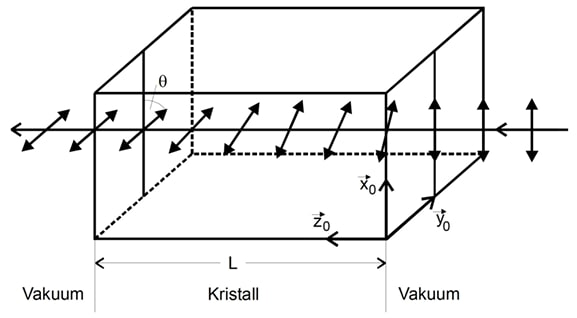
\includegraphics[width=1\textwidth]{content/grafiken/kristall.JPG}
    \caption{Drehung der Polarisationsebene einer elekromagnetischen Welle im B-Feld durchfluteten Medium. [1]}
    \label{fig:kristall}
  \end{figure}